% !TeX encoding = UTF-8
% !TeX spellcheck = it_IT

\documentclass[
	a4paper,
	11pt,
	oneside
]{book}

\usepackage[utf8]{inputenc}
\usepackage[T1]{fontenc}
\usepackage[italian]{babel}

\usepackage[
	left = 0.8in,
	right = 0.8in,
	top = 1in,
	bottom = 1in
]{geometry}

\usepackage{hyperref}
\usepackage{amsmath}
\usepackage{amssymb}
\usepackage{amsthm}
\usepackage{thmtools}
\usepackage{graphicx}
\usepackage{float}
\usepackage{tikz}
\usetikzlibrary{shapes.geometric}
\usetikzlibrary{positioning}
\usetikzlibrary{shapes.arrows}

\graphicspath{ {./images/} }

\newtheoremstyle{std}% name
{}%         Space above, empty = `usual value'
{}%         Space below
{\normalfont}% Body font
{}%         Indent amount (empty = no indent, \parindent = para indent)
{\bfseries}% Thm head font
{}%        Punctuation after thm head
{\newline}% Space after thm head: \newline = linebreak
{}%			Thm head spec

\theoremstyle{std}
\declaretheorem[
	name = {Definizione},
	style = std,
	qed = $ \lozenge $,
	numberwithin = chapter
]{definition}

\title{
\includegraphics[height = 2.5cm]{units.png} \\[0.5cm]
	{\LARGE Università degli Studi di Trieste} \\
	{\Large Dipartimento di Matematica e Informatica} \\[3cm]
	{\large Appunti di}\\ Introduzione al Machine Learning \\ [2cm]
	{\large A.A. 2024-25}}
\author{Ludovico Urbani\\ SM3201372}

\begin{document}
	\pagenumbering{roman}
	\maketitle
	\tableofcontents
	\pagebreak
	\pagenumbering{arabic}
	
	\part{Teoria}
	
	\chapter{Introduzione}
	Il machine learning è una parte dell'intelligenza artificiale che si occupa della costruzione di metodi che imparano, cioè di metodi che utilizzano i dati per migliorare le prestazioni di una serie di compiti. \\
	L'intelligenza artificiale può risolvere problemi o prendere decisioni che tradizionalmente hanno bisogno dell'intervento umano; in particolare il machine learning impara autonomamente senza essere esplicitamente programmato con delle regole. Cioè a differenza della data scienze classica, utilizza i dati per dedurre gli algoritmi.
	\begin{center}
		\begin{tikzpicture}
			\node at (0, 1) [] {Computer science};
			\node at (0, 0) [regular polygon, regular polygon sides=4, draw] (pc1) {$ PC $};
			\node at (-3, 0.3) [] (data1) {Data};
			\node at (-3, -0.3) [] (program1) {Program};
			\node at (3, 0) [] (out1) {Output};
			\draw [-stealth, ultra thick](data1) -- (-1, 0.3);
			\draw [-stealth, ultra thick](program1) -- (-1, -0.3);
			\draw [stealth-, ultra thick](out1) -- (1, 0);
		\end{tikzpicture} \hspace{1cm}
		\begin{tikzpicture}
			\node at (0, 1) [] {Machine learning};
			\node at (0, 0) [regular polygon, regular polygon sides=4, draw] (pc1) {$ PC $};
			\node at (-3, 0.3) [] (data1) {Data};
			\node at (-3, -0.3) [] (out1) {Output};
			\node at (3, 0) [] (program1) {Program};
			\draw [-stealth, ultra thick](data1) -- (-1, 0.3);
			\draw [-stealth, ultra thick](out1) -- (-1, -0.3);
			\draw [stealth-, ultra thick](program1) -- (1, 0);
		\end{tikzpicture}
	\end{center}
	
	\section{Tipi di modelli}
	Esistono tre tipi principali di modelli di machine learning:
	\begin{enumerate}
		\item Supervised learning
		\item Unsupervised learning
		\item Reinforcement learning
	\end{enumerate}
	% TODO immagine schema tre tipi + schema albero classificazioni
	\begin{definition}[Task e modello]
		Un task (compito o attività) è un problema specifico che un sistema di intelligenza artificiale cerca di risolvere. Rappresenta l'obiettivo finale per il quale si addestrano i modelli. I task possono variare ampiamente, come classificare immagini, tradurre testi, riconoscere il parlato o generare testo. \\
		Un modello è un algoritmo matematico o una rete neurale addestrata per risolvere un particolare task. Il modello apprende dai dati di addestramento per fare previsioni o prendere decisioni in base a nuove informazioni. Il modello è quindi lo strumento o l'implementazione che viene utilizzata per risolvere il task. \\
		In sintesi, un task rappresenta ciò che si desidera ottenere o risolvere, mentre un modello è lo strumento concreto che apprende e viene utilizzato per raggiungere il risultato di quel task.
	\end{definition}
	
	\section{Gli input}
	\begin{definition}[Data space]
		I dati di training sono formati da coppie $ (\textbf{x}, y) $, dove $ \textbf{x} \in \mathbb{R}^d $ è l'input e $ y $ l'etichetta. L'intero dataset di training è denotato come:
		$$
			D = \{(\textbf{x}_1, y_1), \ldots, (\textbf{x}_n, y_n)\} \subseteq \mathbb{R}^d \prod \mathcal{C}
		$$
		dove:
		\begin{itemize}
			\item $ \mathbb{R}^d $ è lo spazio d-dimensionale delle caratteristiche
			\item $ \textbf{x}_i $ è il vettore input
			\item $ y_i $ è l'etichetta
			\item $ \mathcal{C} $ è lo spazio delle etichette
		\end{itemize}
		I punti dati $ (\textbf{x}_i, y_i) $ sono estratti da una distribuzione (sconosciuta) $ \mathcal{P}(X, Y) $. \\
		In definitiva, vorremmo imparare una funzione $ h $ tale che per una nuova coppia $ (\textbf{x}, y) \sim P $, si abbia $ h(\textbf{x}) = y $ con alta probabilità (o $ h(\textbf{x}) \approx y $).
	\end{definition}
	Gli scenari per lo spazio delle etichette $ \mathcal{C} $ possono essere:
	\begin{itemize}
		\item Classificazione binaria: $ \mathcal{C} \in \{0, 1\} $ o $ \mathcal{C} \in \{-1, +1\} $
		\item Classificazione multi-classe: $ \mathcal{C} \in \{1, 2, \ldots K\} $ con $ K \geq 2 $
		\item Regressione: $ \mathcal{C} = \mathbb{R} $
	\end{itemize}
	
	\subsection{One hot encoding}
	La maggior parte dei set di dati reali presentano colonne di tipo misto. Questi set di dati sono costituiti da colonne sia categoriche che numeriche. Tuttavia, diversi modelli di apprendimento automatico non funzionano con i dati categoriali e per inserirli nel modello di apprendimento automatico devono essere convertiti in dati numerici. \\
	Il one hot encoding è una tecnica utilizzata per rappresentare le variabili categoriali come valori numerici in un modello di apprendimento automatico. La variabile categoriale viene separata in più colonne, una per ogni possibile valore della variabile categoriale. I valori di queste colonne vengono settati a $ 0 $, tranne per la colonna corrispondente alla categoria selezionata (vedi \autoref{figure:introduzione.input.onehot}). \\
	\begin{figure}[h]
		\centering
		\begin{tabular}{c}
			\textbf{Colori} \\
			Rosso \\
			Rosso \\
			Giallo \\
			Verde \\
			Giallo
		\end{tabular} \hspace{1cm} $ \Longrightarrow $ \hspace{1cm} \begin{tabular}{c c c}
			\textbf{Rosso} & \textbf{Giallo} & \textbf{Verde} \\
			1 & 0 & 0 \\
			1 & 0 & 0 \\
			0 & 1 & 0 \\
			0 & 0 & 1 \\
			0 & 1 & 0
		\end{tabular}
		\caption{One hot encoding}
		\label{figure:introduzione.input.onehot}
	\end{figure}
	I vantaggi di questa tecnica sono:
	\begin{itemize}
		\item Permette di utilizzare variabili categoriche in modelli che richiedono input numerici.
		\item Può migliorare le prestazioni del modello fornendo al modello maggiori informazioni sulla variabile categorica.
		\item Può aiutare a evitare il problema dell'ordinabilità, che può verificarsi quando una variabile categorica ha un ordinamento naturale (es. “piccolo”, “medio”, “grande”).
	\end{itemize}
	Gli svantaggi sono:
	\begin{itemize}
		\item Può portare a un aumento della dimensionalità, poiché viene creata una colonna separata per ogni categoria della variabile. Questo può rendere il modello più complesso e lento da addestrare.
		\item Può portare a dati scarsi, poiché la maggior parte delle osservazioni avrà un valore 0 nella maggior parte delle colonne codificate a un punto.
		\item Può portare a un overfitting, soprattutto se le categorie della variabile sono numerose e la dimensione del campione è relativamente piccola.
	\end{itemize}
	La codifica one-hot è una tecnica potente per trattare i dati categoriali, ma può portare a un aumento della dimensionalità, della sparsità e a un overfitting. È importante utilizzarla con cautela e prendere in considerazione altri metodi, come la codifica ordinale o la codifica binaria.
	
	\subsection{Suddivisione del dataset}
	Il dataset viene suddiviso in:
	\begin{itemize}
		\item Training-set
			\begin{itemize}
				\item Training data: usato per apprendere i parametri del modello
				\item Validation data: usato per decidere che modello usare e quale regolarizzazione funziona meglio (non viene usato per apprendere)
			\end{itemize}
		\item Testing-set: usato alla fine per ottenere quanto buono è il modello, stimato senza bias.
	\end{itemize}
	\begin{figure}[h]
		\centering
		\begin{tikzpicture}
			\begin{scope}[local bounding box=group]
				\node[draw, minimum width = 5cm] (train) {Train};
				\node[draw, minimum width = 2cm, right = 0cm of train] (validation) {Validation};
				\node[draw, minimum width = 2cm, right = 1cm of validation] (test) {Test};
			\end{scope}
			\node[draw, minimum width = 9cm, above = 2cm of group] (dataset) {Dataset};
			\node[single arrow, draw, minimum width = 0.3cm, minimum height = 1.5cm, rotate = 270, below = 1cm of dataset, anchor = center] {};
		\end{tikzpicture}
		\caption{Suddivisione del dataset}
	\end{figure}
	
	\chapter{Fitting}
	La capacità di prevedere bene si dice generalizzazione.
	\begin{figure}[h]
		\centering
		\begin{tikzpicture}[node distance = 1cm]
			\node[align = center] (findf) {find $ \hat{f} \in \mathcal{F} $ \\ s.t. $ y_i \approx \hat{f}(x_i) $};
			\node[left = of findf] () {Learning};
			\node[align = center, above left = of findf] (functions) {Functions $ \mathcal{F} $ \\ $ f : \mathcal{X} \rightarrow \mathcal{Y} $};
			\path[->] (functions.south) edge (findf);
			\node[align = center, above right = of findf] (trainset) {Training data \\ $ \{(x_i, y_i) \in \mathcal{X} \times \mathcal{Y}\} $};
			\path[->] (trainset.south) edge (findf);
			\node[below = of findf] (y) {$ y = \hat{f}(x) $};
			\path[->] (findf) edge (y);
			\node[right = of y] (x) {New data $ x $};
			\path[->] (x) edge (y);
			\node[left = of y] () {Prediction};
		\end{tikzpicture}
		\caption{Schema del processo di supervised learning}
	\end{figure}
	
	\section{La regressione lineare}
	Facciamo l'ipotesi che la relazione tra input e output sia lineare e ci poniamo le domande: come otteniamo/impariamo la linea interpolante? e quanto "buono" è il modello.\\
	Per sapere se il modello lineare è una buona scelta, bisogna conoscere i \textit{priors} del fenomeno studiato.
	\begin{definition}[Loss]
		Dato il dataset $ \{(\textbf{x}_1, y_1), \ldots, (\textbf{x}_n, y_n)\} $ e vettore $ w $ dei pesi del modello lineare. Definiamo i valori predetti dal modello per la variabile target $ y $ come:
		$$
			\hat{y} = w^T x + b
		$$
		Allora possiamo definire la funzione Loss (orrore di predizione) come:
		$$
			\mathcal{L}(w, b) = \frac{1}{N} \sum_{i=1}^N \left(y_i - \left(w^T x_i + b\right)\right)^2 = \frac{1}{N} \sum_{i=1}^N \left(y_i - \hat{y}_i\right)^2
		$$
	\end{definition}
	Alternative alla funzione Loss sono:
	\begin{itemize}
		\item Regressione lineare:
			$$
				\frac{1}{N} \sum_{i=1}^N \left(y_i - \left(w^T x_i + w_0\right)\right)^2
			$$
		\item Regressione logistica:
			$$
			\frac{1}{N} \sum_{i=1}^N \log\left(1 + e^{-y_i \left(w^T G_i + w_0\right)}\right)
			$$
		\item Macchina a vettori di supporto (SVM):
			$$
			\frac{1}{N} \sum_{i=1}^N \max\left(0, -y_i \left(w^T x_i + w_0\right)\right)
			$$
	\end{itemize}
	
	\section{Adattamento della curva polinomiale}
	\begin{definition}[Loss]
		\label{definition:fitting.polynomial.loss}
		Dato il dataset $ \{(\textbf{x}_1, y_1), \ldots, (\textbf{x}_n, y_n)\} $ e vettore $ w $ dei pesi del modello.
		La funzione loss per una regressione alla curva polinomiale misura gli errori quadrati della variazione tra i dati reali e i valori predetti.
		$$
			E(\textbf{w}) = \frac{1}{2} \sum_{i=1}^N \left(y(x_i, \textbf{w}) - y_i\right)^2
		$$
		con $ y $ regressione polinomiale definita come:
		$$
			y(x, \textbf{w}) = w_0 + w_1 x + w_2 x^2 + \ldots + w_M x^M
			= \sum_{i=0}^M w_i x^i
		$$
	\end{definition}
	\begin{figure}[H]
		\centering
		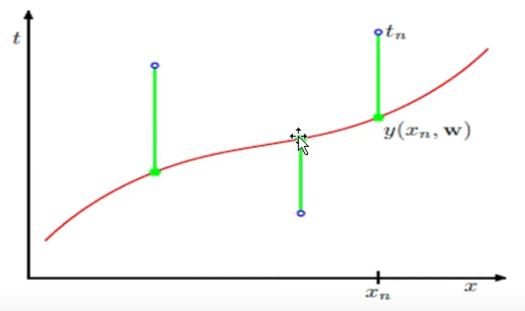
\includegraphics[width = 8cm]{polynomial_loss.png}
		\caption{Loss di una regressione polinomiale}
	\end{figure}
	
	\subsection{Overfitting}
	\begin{definition}[Overfitting]
		Definiamo l'overfitting nella regressione polinomiale quando il grado del polinomio è così alto che il modello diventa troppo complesso, riuscendo a seguire ogni piccola variazione dei dati di addestramento. Di conseguenza, il modello perde la capacità di generalizzare su nuovi dati e diventa inefficace per fare previsioni affidabili.
	\end{definition}
	\begin{figure}[H]
		\centering
		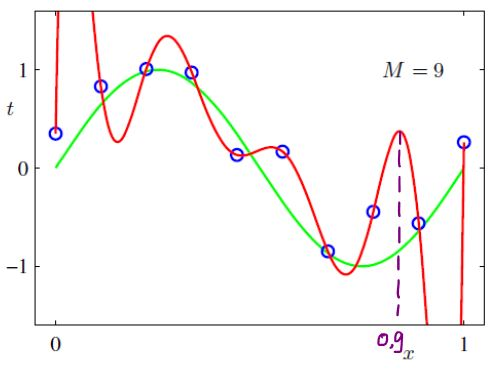
\includegraphics[width = 8cm]{overfitting.jpg}
		\caption{Overfitting}
	\end{figure}
	\begin{definition}[Root mean square error (RMS)]
		Definiamo l'errore quadratico medio (EQM) come:
		$$
			E_{RMS} = \sqrt{\frac{2}{N} E(w^*)}
		$$
	\end{definition}
	L'overfitting si verifica quando l'errore di training va a zero, ma l'errore nei test cresce insieme al grado del polinomio.
	\begin{figure}[H]
		\centering
		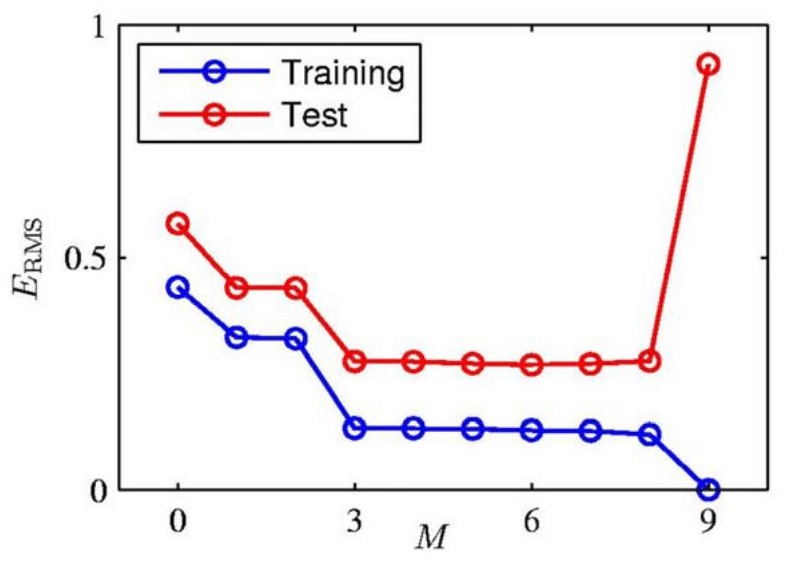
\includegraphics[width = 8cm]{overfitting_rms.png}
		\caption{Remazione overfitting-RMS}
	\end{figure}
	Se il modello ha tanti gradi di libertà quanti sono i dati, può adattarsi perfettamente ai dati di addestramento, ma l'obiettivo del ML è la generalizzazione. Quindi ci si può aspettare che un modello generalizzi bene se spiega i dati di addestramento bene data la complessità del modello.\\
	Per prevenire l'overfitting si deve aumentare il numero di dati di input, oppure diminuire il numero di gradi di libertà della curva.
	Come mostrato nella \autoref{figure:fitting.polynomial.overfitting.coeff} è possibile (non sempre) verificare la presenza di overfitting osservando i valori dei pesi $ w_i $: quando i valori "esplodono" in grandezza, è possibile la presenza di overfitting.
	\begin{figure}[h]
		\centering
		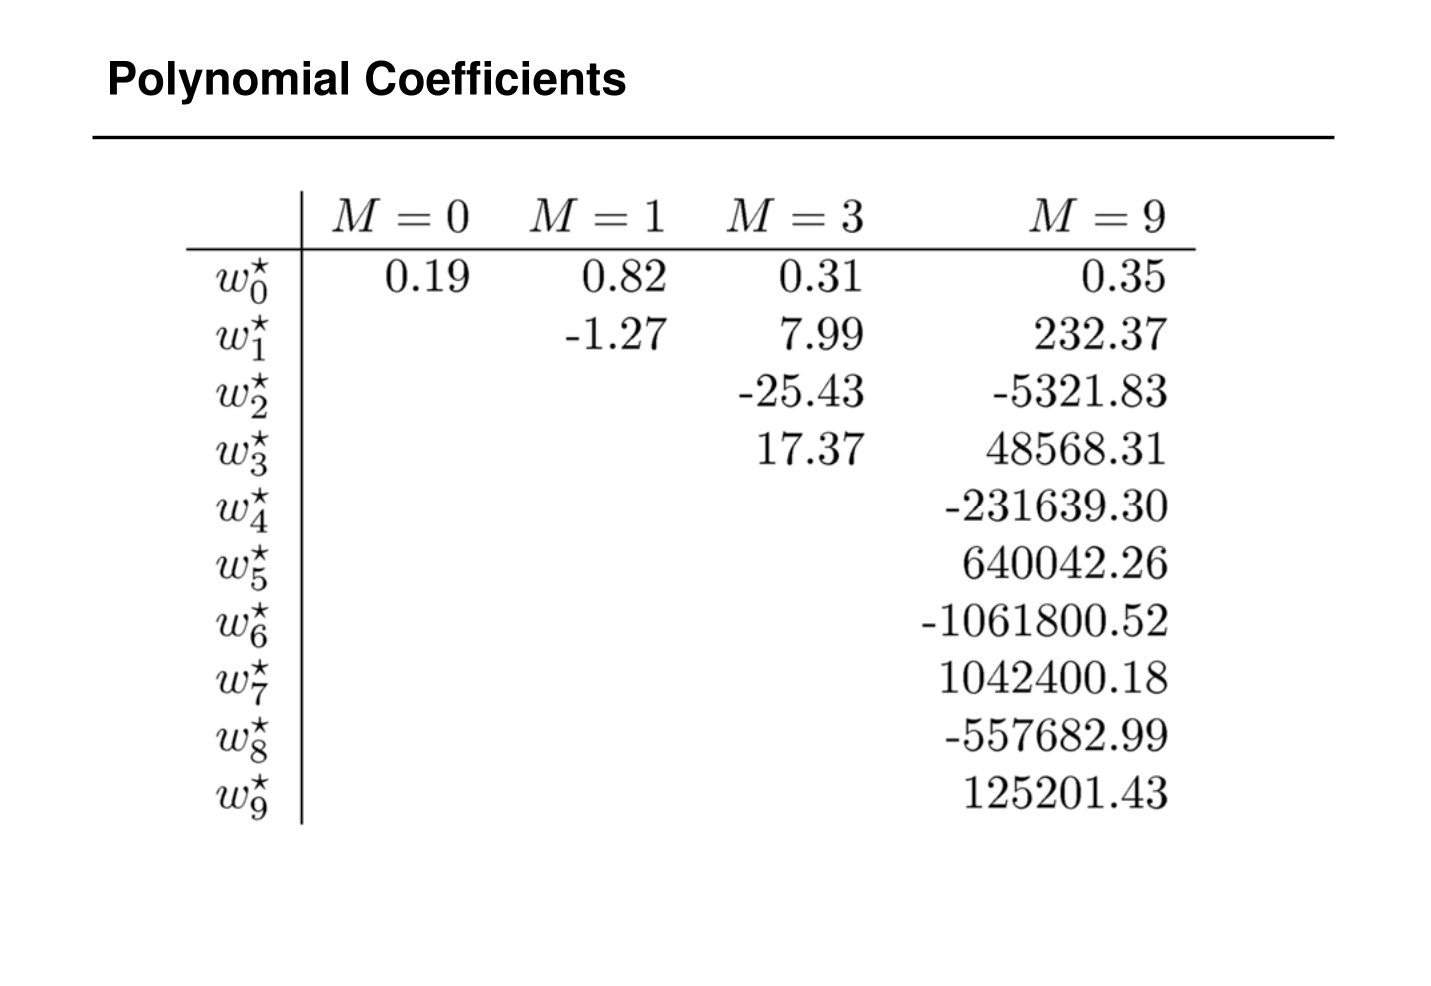
\includegraphics[width = 8cm]{overfitting_coeff.png}
		\caption{Coefficienti polinomiali}
		\label{figure:fitting.polynomial.overfitting.coeff}
	\end{figure}
	Un altro metodo per prevenire l'overfitting è di applicare una regolarizzazione della funzione di Loss, cioè penalizzare i coefficienti grandi.
	\begin{definition}[Loss con regolarizzazione]
		Nelle ipotesi della \autoref{definition:fitting.polynomial.loss}, definiamo la funzione di Loss con regolarizzazione come:
		$$
			\tilde{E} = \frac{1}{2} \sum_{i=1}^N \left(y(x_i, \textbf{w}) -y_i\right)^2 + \frac{\lambda}{2} \lVert \textbf{w} \rVert^2
		$$
		dove $ \lVert \textbf{w} \rVert^2 $ è la norma L2-quadro e $ \lambda $ è l'iperparametro scelto in partenza.
	\end{definition}
	
	\part{Laboratorio}
	
\end{document}